\section{Durchführung}
\label{sec:Durchführung}
Für die Messung der Suszeptibilität wird der in \autoref{fig:blockschaltbild} dargestellte Aufbau verwendet.

\begin{figure}[H]
	\centering
	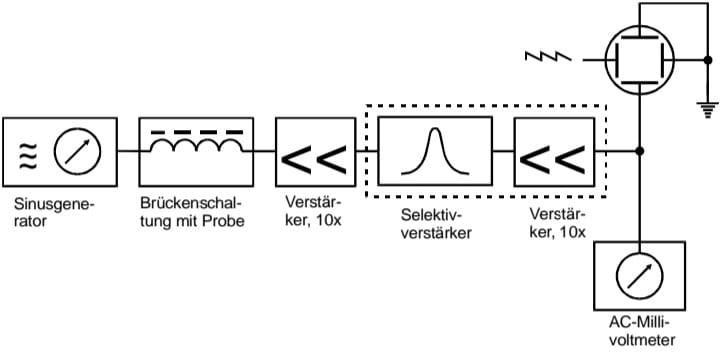
\includegraphics[width=0.6\linewidth]{data/blockschaltbild.jpeg}
	\caption{Blockschaltbild der verwendeten Messapparatur \cite{Anleitung606}.}
	\label{fig:blockschaltbild}
\end{figure}
\noindent
Da zur Messung eine Brückenschaltung verwendet wird, ensteht an den Ausgängen eine Störspannung, die die eigentliche Brückenspannung komplett überdeckt. Um die Brückenspannung
trotzdem messbar zu machen wird ein Selektivverstärker verwendet, der nur für monofrequente Signalspannungen durchlässsig ist und somit die Brückenspannung herausfiltert. Es wird 
außerdem ein Linearverstärker verwendet, um die kleinen Spannungsänderungen messbar zu machen.
\newline \newline
Im ersten Schritt der Messung wird die Filterkurve des Selektivfilters bestimmt. Hierzu wird die Spannungsquelle direkt mit dem Selektivverstärker verbuden. Es kann nun die Spannungsfrequenz
variiert und die daraus resultierende Ausgangsspannung $U_{\text{A}}$ mit Hilfe eines Millivoltmeters gemessen und notiert werden. Die Messungen wurden in einen Frequenzbereich von 20 bis
$\SI{40}{\kilo\hertz}$ durchgeführt, wobei die Abstände der Messwerte nahe des Peaks der Ausgangsspannung $U_{\text{A}}$ enger gewählt wurden als am Rand des Frequenzbereichs.
\newline \newline
Im zweiten Schritt des Versuches wird nun die eigentliche Suszeptibilitätsmessung durchgeführt. Hierfür wird zunächst die Signalfrequenz auf die Durchlassfrequenz des Selektivverstärkers
eingestellt. Zur Messung werden zwei verschiedene Methoden angewandt. Zum einen wird die Änderung der Brückenspannung gemessen, die auftritt, wenn bei abgeglichener Brücke mit leeren Spulen
die Probe in diese eingeführt wird. Zum anderen wird die Brücke nach Einführung der Probe erneut abgeglichen und die veränderten Werte der Widerstände notiert.
\newline
Beide Verfahren werden jeweils parallel für die drei zu messenden Seltenen Erd-Oxiden $Gd_2O_3$, $Nd_2O_3$ und $Dy_2O_3$ angewandt. Es wird jede Messung drei mal durchgeführt und aus den
Ergebnissen jeweils der Durchschnitt gebildet. Anschließend werden die Längen und Durchmesser der Proben vermesssen.